% ------------------------------------------------------------------------
%                             Capítulo 4
% ------------------------------------------------------------------------
\chapter{Implementación en C++}

Este capítulo trata el proceso de traducción del código de Matlab a C++ mediante las funciones de la librería gráfica OpenCV. La mayor parte del trabajo es una traducción directa, debido a que la mayoría de las funciones utilizadas en Matlab tienen un equivalente en OpenCV. 

Una explicación detallada del proceso consistiría esencialmente en volver sobre lo tratado en el capítulo anterior. Por tanto este capítulo sé centrará en las mayores diferencias entre las dos implementaciones; así como los problemas encontrados en el proceso.

\section{Algoritmo de Canny}
La primera diferencia reside en el algoritmo de Canny. La implementación y la parametrización que utiliza OpenCV es diferente a la que utiliza Matlab. Además, la rutina de Matlab implementa el filtrado gaussiano en la misma rutina que el algoritmo de Canny; mientras que en OpenCV es necesario utilizar dos rutinas diferentes.\\

\begin{figure}[!h]
\centering 
\subfigure[Matlab]{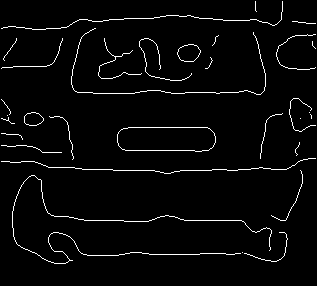
\includegraphics[width=6cm]{EjemploCanny.png}}
\subfigure[OpenCV]{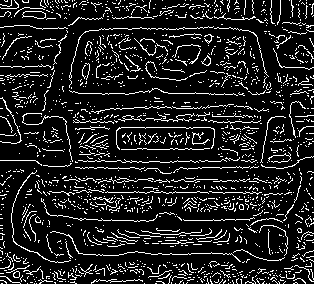
\includegraphics[width=6cm]{CannyOpenCV1.png}}
\caption{\small{Resultado del algoritmo con los mismos parámetros.}} \label{CannyOpenCV}
\end{figure}

En la \reff{CannyOpenCV} pueden observarse los diferentes resultados que produce el algoritmo de Canny en Matlab y OpenCV usando los mismos parámetros. La imagen (a) muestra el resultado del algoritmo de Canny en Matlab, tal y como se vio en \ref{Canny}; mientras que en la imagen (b) se observa el resultado del algoritmo en OpenCV utilizando los mismos parámetros.\\


Resulta evidente que este resultado no es aceptable, por lo que es necesario volver a calcular los parámetros del algoritmo.\\

Durante este proceso de parametrización se llegó a la conclusión de que se pueden conseguir resultados interesantes utilizando diferentes valores de desviación típica en el filtro gausiano para los ejes $x$ e $y$, lo cual es posible gracias a que la rutina de filtro gausiano utilizada en OpenCV lo permite.\\


\begin{figure}[!h]
\centering 
\subfigure[Misma desviación típica.]{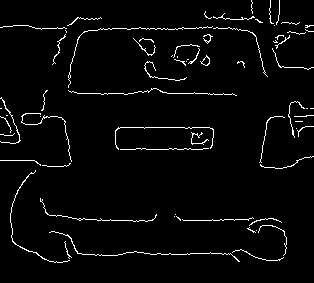
\includegraphics[width=6cm]{CannyOpenCV2.png}}
\subfigure[Distinta desviación típica.]{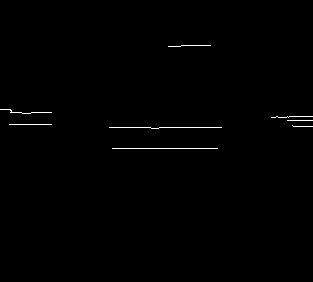
\includegraphics[width=6cm]{CannyOpenCV3.png}}
\caption{\small{Efecto de usar distintas desviaciones tipicas en los ejes.}} \label{CannyOpenCV2}
\end{figure}

En la \reff{CannyOpenCV2}, se observa un ejemplo de esta idea. La imagen (a) representa el resultado del algoritmo de Canny, donde se ha empleado la misma desviación típica en los dos ejes y una parametrización que consigue resultados similares a los obtenidos con Matlab en el apartado \ref{Canny}. La imagen (b) muestra el resultado tras aplicar una desviación típica mayor en el eje $x$ que en el $y$. \\

Lo que ocurre en la imagen (b) se debe a que el filtro distorsiona completamente los contornos verticales, dejando los horizontales intactos. Esto simplifica enormemente el trabajo de encontrar las líneas de la matrícula, ya que los candidatos a matrícula se reducen en gran medida.\\

El código C++ utilizado para realizar el algoritmo es el siguiente:

\begin{lstlisting}
GaussianBlur( ImgOriginal, ImgFiltrada, DimFiltro, sigmax, sigmay);
Canny(ImgFiltrada, ImgContornos, T1, T2);
\end{lstlisting}

Donde:
\begin{itemize}
\item \textbf{DimFiltro} es el parámetro que configura la dimensión del kernel usado por el filtro. En esta aplicación se ha configurado con tamaño 0 para que la función decida el tamaño.
\item \textbf{sigmax y sigmay} se corresponden con las desviaciones típicas usadas en los ejes $x$ e $y$ respectivamente. En esta aplicación se configuran con $sigmax=10$ y \\$ sigmay=1$.
\item\textbf {T1 y T2} se corresponden con los umbrales usados por el algoritmo para determinar los contornos. En esta aplicación se eligen como valores $T1=100$ y $T2=250$.
\end{itemize}

\section{Transformada de Hough}\label{CannyCV}
Otra diferencia la encontramos en la transformada de Hough.\\

OpenCV cuenta con una función que busca directamente las líneas rectas en una imagen usando la transformada de Hough:


\begin{lstlisting}
HoughLinesP(ImgContornos, lines, rho, theta, th, minLength, maxGap );
\end{lstlisting}

Donde:
\begin{itemize}
\item \textbf{lines} es una estructura donde se almacenan las líneas encontradas.

\item \textbf{rho y theta} se corresponden con la sensibilidad usada en los eje rho y theta para calcular las líneas. En esta aplicación se configuran como $tho=w/300$ (píxeles) y $ theta=1º$.

\item\textbf {th} indica el número de líneas que deben coincidir en un punto en el plano $ab$ para ser considerado línea. En esta aplicación se usará $th = anchoImg/10$.

\item\textbf{minLength} indica la longitud mínima en píxeles que debe tener una línea para ser considerada. Para esta aplicación se usará $minLength~=~anchoImg/5$.

\item\textbf{maxGap} establece la discontinuidad máxima que puede contener una línea para que no sea considerada como dos líneas distintas. En esta aplicación se utilizara\\ $maxGap~=~anchoImg/10$.
\end{itemize}

En el parámetro \textbf {th} se halla la primera diferencia respecto a Matlab. En la implementación en Matlab se tiene acceso directo a la matriz \textbf{H}, como se vio en el apartado \ref{Hough}, lo que hace posible configurar \textbf {th} en función del máximo de \textbf{H}.\\

Otro problema encontrado es el que se ilustra en la \reff{ProblemaLineasOpenCV}.\\

\begin{figure}[!h]
\centering \subfigure[Resultado del algoritmo de Canny.]{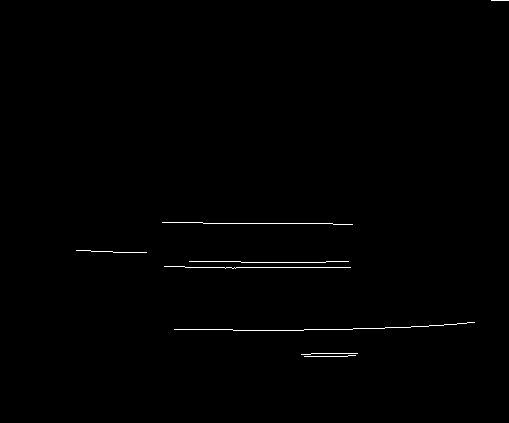
\includegraphics[width=6cm]{ProblemaCannyOpenCV.png}}
\subfigure[Líneas encontradas.]{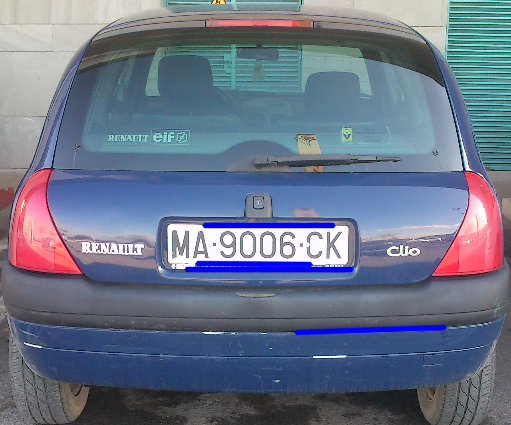
\includegraphics[width=6cm]{ProblemaLineasOpenCV.png}}
\caption{\small{Problemas con la detección de líneas.}} \label{ProblemaLineasOpenCV}
\end{figure}

La imagen (a) muestra el resultado del algoritmo de Canny, donde se muestran todos los contornos detectados en la imagen. Entre ellos se encuentran los dos contornos correspondientes a la matrícula con pequeñas imperfecciones. En la imagen (b) se observan las líneas encontradas por la función. Puede observarse cómo el algoritmo no ha reconocido la línea completa debido a las imperfecciones.\\

La solución a este problema consiste en reducir la sensibilidad usada por el algoritmo mediante los parámetros \textbf{rho} y \textbf{theta}; pero el resultado obtenido no se corresponde con el esperado. La reducción de la sensibilidad no produce ninguna mejora en absoluto, y no se ha encontrado ninguna combinación de parámetros que consiga solucionar el problema.\\

Encontrar una solución definitiva para el problema pasa por investigar la implemtentación que realiza OpenCV de la transformada de Hought, para modificarla o realizar pruebas con otras funciones de transformada de Hough disponibles de forma libre. No obstante, la duración de este \ac{TFG} no permite la realización de estas pruebas.